\documentclass[12pt]{article}
\usepackage[left = 1in, right = 1in, top = 1in, bottom = 1in]{geometry}
\usepackage{paralist}
\usepackage{enumitem}
\usepackage{amsmath}
\usepackage{amssymb}
\usepackage{amsthm}
\usepackage{tikz}
\usepackage{hyperref}
\usepackage{esdiff}
\usepackage{parskip}

\begin{document}

\section{Definition}

We define a derivative of a function $f(x)$ with respect to $x$ as

\[\diff{f}{x} = \lim_{h\to_{0}} \frac{f(x + h) - f(x)}{h}\]

At $x = 0$, if $f$ is differentiable, then limit as $h \to 0^{+}$ must 
equal the limit as $h \to 0^{-}$.

\section{Differentiation Rules}

\noindent Chain Rule: If $f(x) = F(g(x))$, then
\[f'(x) = \diff Fg \diff gx\]

\noindent Product Rule: If $f(x) = u(x)v(x)$, then
\[f'(x) = u'(x)v(x) + u(x)v'(x)\]

\noindent Quotient Rule: 
If $f(x) = \frac{u(x)}{v(x)}$, then
\[f'(x) = \frac{1}{(v(x))^{2}}(u'(x)v(x) - u(x)v'(x))\]

\noindent L'Hopital Rule: If $\lim_{x \to x_{0}} f(x) = \lim_{x \to x_{0}} g(x)$, then
\[\lim_{x\to x_{0}} \frac{f(x)}{g(x)} = \lim_{x\to x_{0}} \frac{f'(x)}{g'(x)}\]

\section{Sidenote: Big O and litle o notation}

We say that a function $H(x) = o(g(x))$ as $x \to x_{0}$ if
\[\lim_{x\to x_{0}} \frac{H(x)}{g(x)} = 0.\]

\noindent We say that a function $H(x) = O(g(x))$ as $x \to x_{0}$ if
\[\lim_{x\to x_{0}} \frac{H(x)}{g(x)} = C\]
for some constant $C \in \mathbb{R}$.

\section{Functions of several variables}

Consider a function $f(x,y)$ in two-dimensional space.
For example, $f$ could describe a contour on some terrain.

We find the slopes in directions parallel directions to the axes $x,y$
by defining partial derivatives of $f(x,y)$ with respect to $x$ or $y$.

We define the partial derive of $f(x,y)$ with respect to $x$ as
the rate of change of $f$ as we vary $x$ but keeping $y$ constant. We write
\[
    \left.\frac{\partial f}{\partial x}\right|_y 
        = \lim_{\delta x \to 0}\left[\frac{f(x + \delta x, y) - f(x,y)}{\delta x}\right]
\]

\[
    \left.\frac{\partial f}{\partial y}\right|_x 
        = \lim_{\delta y \to 0}\left[\frac{f(x, y + \delta y) - f(x,y)}{\delta y}\right]
\]

For example, let, $f(x,y) = x^{2} + y^{3} + e^{xy^{2}}$. Then,

\[ \begin{aligned}
    \left.\diffp f x\right |_{y} &= 2x + 0 + y^{2}e^{xy^{2}} \\
    \left.\diffp f y\right |_{x} &= 0 + 3y^{2} +  2xy e^{xy^{2}} \\
    \left.\diffp[2] f x\right |_{y} &= 2 + 0 + y^{4}e^{xy^{2}} \\
\end{aligned} \]

We can extend this definition to functions of arbitrary many variables.
For example, let $f(x_{1},x_{2},\cdots x_{n})$, we can say that the partial derivative of
$f$ wrt $x_{i}$ is

\[\left.\diffp f x_i\right|_{x_{1},x_{2}, \cdots x_{i-1}, x_{i+1},\cdots x_{n}}\]

\subsection{Total Derivatives}

Consider a change in $f$, let $\delta f = f(x + \delta x, y + \delta y) - f(x,y)$.
We can write this change as

\[
    \begin{aligned}
        \delta f &= f(x + \delta x,y+\delta y) &- f(x + \delta x,y) \\
                 &+ f(x + \delta x,y) &- f(x,y) \\
            &= \left.\diffp f y\right|_{x} (x + \delta x, y+\delta y)\delta y + o(\delta  y) \\
            &+ \left.\diffp f y\right|_{x} (x, y)\delta x + o(\delta  x)
    \end{aligned}
\]

So by taking the limits $\delta x,\delta y\to 0$ we can say that the total change in $f$ is

\[d f = \left.\diffp f y\right|_{x}d y 
    + \left.\diffp f x\right|_{y}dx\]

\subsection{Chain Rule}

Suppose $f(x,y)=f(X(t),Y(t))$, then we can find the
rate of change of $f$ wrt $t$ by using the above result.

\[\diff{f}{t} = \left.\frac{\partial f}{\partial y}\right|_{x} \diff{y}{t}
    + \left.\frac{\partial f}{\partial x}\right|_{y} \diff{x}{t}\]

Let a path be defined as $y = y(x)$, so parametrized as $x=t,y=y(t)$, then
\[\diff{f}{t} = \left.\diffp f y\right|_{x}\diff yt + \left.\diffp f x\right|_{y}\]

so then
\[\diff{f}{x} = \left.\diffp f y\right|_{x}\diff yx + \left.\diffp f x\right|_{y}\]


\subsection{Change of variables}
Suppose we want to change variables from $x,y$ to $r,\theta$.
So $f(x,y)=F(r,\theta )$, and there are transformations $x=x(r,\theta )$ and $y=y(r,\theta )$.
Then, we can find the derivatives of $F$ wrt $r$ and $\theta $ in terms of the
derivatives of $f$ wrt $x$ and $y$.

\[\left.\diffp{F}{r}\right|_{\theta } = \left.\diffp{f}{x}\right|_{y} 
            \left.\diffp{x}{r}\right|_{\theta } 
            + \left.\diffp{f}{y}\right|_{x} 
            \left.\diffp{y}{r}\right|_{\theta }
\]
similarly,
\[\left.\diffp{F}{\theta }\right|_{r } = \left.\diffp{f}{x}\right|_{y} 
            \left.\diffp{x}{\theta }\right|_{r } 
            + \left.\diffp{f}{y}\right|_{x} 
            \left.\diffp{y}{\theta }\right|_{r }
\]

\subsection{Example: More variables}
Consider a function $F(x,y,z) = \text{const}$.
We can solve this for $z = z(x,y)$,
or equivalently $x = x(y,z)$ or $y = y(x,z)$.
Suppose we write $F(x,y,z) = F(x,y,z(x,y))$.

Using the chain rule,
\[
    \begin{aligned}
    \left.\diffp{F}{x}\right|_{y} 
        &= \left.\diffp{F}{x}\right|_{y,z}\left.\diffp{x}{x}\right|_{y} 
        + \left.\diffp{F}{y}\right|_{x,z}\left.\diffp{y}{x}\right|_{y} 
        + \left.\diffp{F}{z}\right|_{x,y}\left.\diffp{z}{x}\right|_{y} \\
        0 &= \left.\diffp{F}{x}\right|_{y,z}
        + \left.\diffp{F}{z}\right|_{x,y}\left.\diffp{z}{x}\right|_{y} \\
    \end{aligned}
\]

so,
\[
    \left.\diffp{z}{x}\right|_{y} = \frac{-\left.\diffp{F}{x}\right|_{y,z}}{\left.\diffp{F}{z}\right|_{x,y}}
\]

after similar calculation for $x,y$,

\[
    \left.\diffp{x}{y}\right|_{z}\left.\diffp{y}{z}\right|_{x}\left.\diffp{z}{x}\right|_{y} = -1
\]


\section{Solving PDEs}

\subsection{Example 1}

Consider the 1st order wave equation,

\[
    \diffp yt - c \diffp yx = 0.
\]

In this notation, it's written

\[
    \left.\diffp{y}{t}\right|_{x} - c\left.\diffp{y}{x}\right|_{t} = 0
\]

Recalling chain rule for $y(x,t)$

\[
\diff yt = \left.\diffp{y}{x}\right|_{t}\diff xt
        + \left.\diffp{y}{t}\right|_{x}\diff tt
\]

Notice that if $\diff xt = -c$, then $\diff yt = 0$.
That path is described by $x = x_{0} - ct$, and $y = \text{const}$.
This can be rewritten as $y = f(x_{0}) = f(x + ct)$ where $f$ is 
an arbitrary function and $x_{0}$ is a constant.

Alternatively, consider a change of variables $(u,v) = (x + ct, x - ct)$. Then,
\[
\begin{aligned}
    \diffp yt &= \diffp yu \diffp u t + \diffp yv \diffp v t \\
                &= c\diffp yu - c\diffp yv \\
    \diffp yx &= \diffp yu \diffp ux + \diffp yv \diffp vx \\
                &= \diffp yu + \diffp yv
\end{aligned}
\]

Substituting yields
\[
    \begin{aligned}
        c\diffp yu - c\diffp yv - c\left(\diffp yu + \diffp yv\right) &= 0 \\
        -2c\diffp yv &= 0 \\
        \diffp yv &= 0 \\
    \end{aligned}
\]

So $y$ is constant with respect to $v$, but not necessarily $u$, 
so any solution $y = f(u) = f(x + ct)$ for some $f$.

\subsection{Example 2}

Consider the PDE
\[
\diffp yt + 5\diffp yx = e^{-t}
\]
with the initial condition $y(x,0) = e^{-x^{2}}$.

Similar to ODEs, we can separate the PDE into a homogeneous and a particular solution.
Homogeneous solution is $y = f(x - 5t)$, by the last example with $c = -5$.

For the particular solution $y_p$ we notice that the RHS of the PDE only depends on $t$,
and the initial condition is at $t = 0$ and only depends on $x$.
Thus, we consider $y_p = y_p(t)$ and find that $y_p = -e^{-t}$ solves the solution.
Therefore, the general solution is
\[
y(x,t) = f(x - 5t) - e^{-t}.
\]
Using our initial condition $y(x,0) = e^{-x^{2}}$,
\[
y(x,0) = f(x+0) - e^{-0} = f(x) - 1 = e^{-x^2}.
\]
Thus, $f(x) = 1 + e^{-x^{2}}$.
Substituting, the solution to this problem is 
\[
y(x,t) = 1 + e^{-(x-5t)^{2}} - e^{-t}.
\]

\newpage
\subsection{Question 5}

Let $p = p(V,S)$, and $p=p(V,S(V,T))$. Then
\begin{equation}
\begin{aligned}
    \left.\diffp{p}{V}\right|_{T} - \left.\diffp{p}{V}\right|_{S}
            &= \left.\diffp{p}{V}\right|_{S}\left.\diffp{V}{V}\right|_{T}
                    + \left.\diffp{p}{S}\right|_{V}\left.\diffp{S}{V}\right|_{T}
                    - \left.\diffp{p}{V}\right|_{s}\\
            &= \left.\diffp{p}{V}\right|_{S}
                    - \left.\diffp{p}{V}\right|_{s}
                    + \left.\diffp{p}{S}\right|_{V}\left.\diffp{S}{V}\right|_{T}\\
            &= \left.\diffp{p}{S}\right|_{V}\left.\diffp{S}{V}\right|_{T}\\
            &= \left[\left.\diffp{S}{p}\right|_{V}\right]^{-1}\left.\diffp{S}{V}\right|_{T}
\end{aligned}
\end{equation}

Now, define $U$ by $TdS=dU+pdV$. Note the following results:

\begin{equation}
T\left.\diffp{S}{p}\right|_{V} = \left.\diffp{U}{p}\right|_{V} + p\left.\diffp{V}{p}\right|_{V} = \left.\diffp{U}{p}\right|_{V},
\end{equation}
and
\begin{equation}
T\left.\diffp{S}{V}\right|_{T} = \left.\diffp{U}{V}\right|_{T} + p\left.\diffp{V}{V}\right|_{T} = \left.\diffp{U}{V}\right|_{T} + p.
\end{equation}

Then,
\[
\begin{aligned}
    \left.\diffp{\log p}{{\log V}}\right|_{T} - \left.\diffp{\log p}{{\log V}}\right|_{S}
            &= \frac{V}{p}\left(\left.\diffp{p}{V}\right|_{T} - \left.\diffp{p}{V}\right|_{S}\right)\\
            &= \frac{V}{p}\left[\left.\diffp{S}{p}\right|_{V}\right]^{-1} \left.\diffp{S}{V}\right|_{T}\\
            &= \frac{V}{p}\left[\frac{1}{T}\left.\diffp{U}{p}\right|_{V}\right]^{-1} \frac{1}{T}\left(\left.\diffp{U}{V}\right|_{T} + p\right)\\
            &= V\left[T\left.\diffp{p}{U}\right|_{V}\right] \frac{1}{T}\left(p^{-1}\left.\diffp{U}{V}\right|_{T} + 1\right)\\
            &= V\left.\diffp{p}{T}\right|_{V}\left.\diffp{T}{U}\right|_{V} \left(p^{-1}\left.\diffp{U}{V}\right|_{T} + 1\right)\\
            &= \left.\diffp{pV}{T}\right|_{V} \left[\frac{p^{-1}\left.\diffp{U}{V}\right|_{T} + 1}{\left.\diffp{U}{T}\right|_{V}}\right]\\
\end{aligned}
\]

\newpage
\subsection{Question 6}

Solve the following equation by change of variable:
\[
    \diffp[2]yt = c^{2}\diffp[2]yx
\]
Let $(u,v) = (x+ct,x-ct)$.

\[
    \diffp[2]yx = \diffp{}x\diffp yx
\]
let $g = \diffp yx$, then

\[
    \diffp[2]yx = \diffp gx = \diffp gu \diffp ux + \diffp gv \diffp vx = \diffp gu + \diffp gv
\]
similarly, let $h = \diffp yt$,
\[
    \diffp[2]yt = c \diffp hu - c \diffp hv
\]
Now note that
\[
\diffp yu = \diffp yx \diffp xu + \diffp yt \diffp tu = \diffp yx + \frac{1}{c}\diffp yt
\]
and similarly,
\[
\diffp yv = \diffp yx \diffp xv + \diffp yt \diffp tv = \diffp yx - \frac{1}{c}\diffp yt
\]
Anyway, basically some algebra later we get
\[
    \diffp[2]yx = \diffp y{uv} + \frac{1}{2}\left(\diffp[2]yu + \diffp[2]yv\right)
\]
\[
    \diffp[2]yt = c^{2}\left(-\diffp y{uv} + \frac{1}{2}\left(\diffp[2]yu + \diffp[2]yv\right)\right)
\]
Substituting back in the original equation, we have
\[
    \diffp y{uv} = 0
\]
Thus, a general solution of $y$ is of the form $y = p(u) + q(v)$.
Substituting $u,v$ we have $y = p(x + ct) + q(x - ct)$.
Applying the conditions of the initial conditions give
\[
p(x) + q(x) = \frac{1}{1 + x^{2}}
\]

Similarly, using the $\diffp yt$ condition yields
\[
    \diffp pt (x) = \diffp qt (x)
\]
Thus, we have $p(x) = q(x) + c$ for some $c$. Substituting gives
\[
2p(x) + c = \frac{1}{1 + x^{2}}
\]
\[
p(x) = \frac{1}{2(1 + x^{2})} - \frac{c}{2}
\]
Thus, we have the general solution
\[
y = \frac{1}{2(1 + (x + ct)^{2})} + \frac{1}{2(1 + (x - ct)^{2})} - c
\]
The final condition is that $\lim_{x\to \pm\infty} y = 0$. 
This holds for any $t$, so take $t = 0$, then
\[
    \lim_{x\to\pm\infty} \frac{1}{2(1+x)^{2}} + \frac{1}{2(1+x)^{2}} - c
\]
solving trivially yields $c = 0$, so
\[
y = \frac{1}{2(1 + (x + ct)^{2})} + \frac{1}{2(1 + (x - ct)^{2})}
\]
Graphing this yields two "lumps", which are clearly moving away,
with centres at $-ct$ and $ct$ respectively.

\begin{figure}[h]
    \centering
    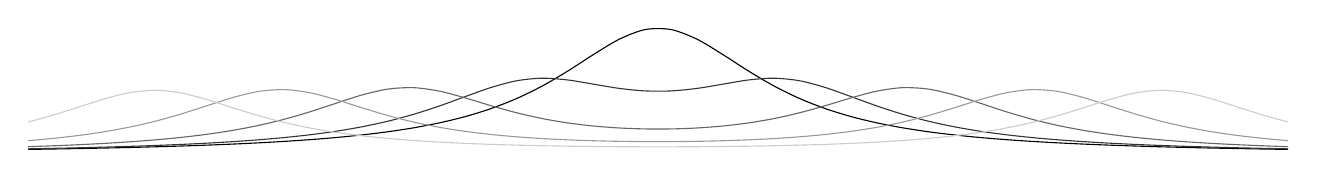
\begin{tikzpicture}[smooth,samples=50,scale=1.6]
        \draw[color=black!100] plot (\x,{1/(\x*\x + 1)});
        \draw[color=black!80] plot (\x,{1/(2 * ((\x - 1)*(\x - 1) + 1)) + 1/(2 * ((\x + 1)*(\x + 1) + 1))});
        \draw[color=black!60] plot (\x,{1/(2 * ((\x - 2)*(\x - 2) + 1)) + 1/(2 * ((\x + 2)*(\x + 2) + 1))});
        \draw[color=black!40] plot (\x,{1/(2 * ((\x - 3)*(\x - 3) + 1)) + 1/(2 * ((\x + 3)*(\x + 3) + 1))});
        \draw[color=black!20] plot (\x,{1/(2 * ((\x - 4)*(\x - 4) + 1)) + 1/(2 * ((\x + 4)*(\x + 4) + 1))});
    \end{tikzpicture}
    \caption{Graph of $y$ for $c=1$ and $t=0,1,2,3,4$}
\end{figure}

\end{document}
